\documentclass[8pt]{beamer}
\usepackage{helvetica,verbatim}
\begin{document}
\title{TIAM+}
\subtitle{extending the Tool for Integrative Analysis of Motility\\ https://github.com/r-medina/TIAM-}
\author{Ricardo Medina}
\date{\today}


\frame{\titlepage}
\frame{\frametitle{Table of contents}\tableofcontents}

\section{Task}
\begin{frame}
  \frametitle{Task}
  Using data from Vivek Mayya and Willie Neiswanger's TIAM tool, which
  performs detection and tracking of cells from multi-channel time
  lapse microscopy videos, build an algorithm that will classify track
  segments. Two initial decisions:
  \begin{itemize}
  \item 2 classes
  \item supervised
  \end{itemize}
  First tasks:
  \begin{itemize}
  \item collect supervised data
  \item engineer/discover useful features for segmented trajectory
    classification
  \end{itemize}
  \begin{columns}
    \begin{column}[t]{0.5\textwidth}
      %video?
    \end{column}

    \begin{column}[t]{0.5\textwidth}
      %video?
    \end{column}
  \end{columns}

\end{frame}

\section{Data Collection}  
\begin{frame}
  \frametitle{GUI}  
  
    \begin{figure}[H]\centering
    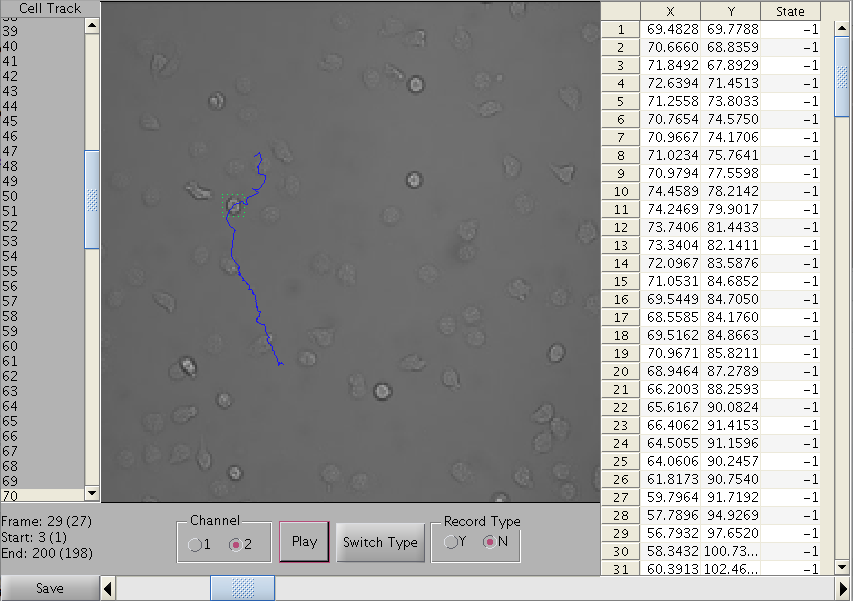
\includegraphics[width=.9\textwidth]{../fig/sc1.png}
  \end{figure}
  
\end{frame}

\begin{frame}
  \frametitle{GUI}  
  
    \begin{figure}[H]\centering
    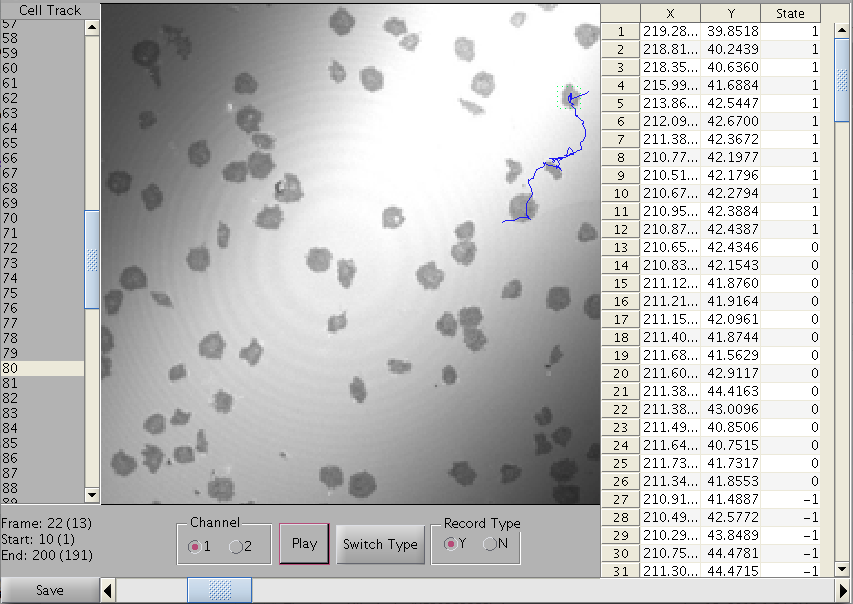
\includegraphics[width=.9\textwidth]{../fig/sc2.png}
  \end{figure}
  
\end{frame}


\section{Building Classifier}

% Look into shape

\begin{frame}
  \frametitle{Features}
  Helmuth \emph{et al.} paper titled ``A novel supervised trajectory
  segmentation algorithm identifies distinct types of human adenovirus
  motion in host cells'' offers a methodology (features and procedure)
  for classifying segments of cell tracks.
  The features for some trajectory part $P_j$ of $l_w$ steps are:
  %{\small
  \begin{itemize}
  \item Net displacement
  \item Straightness
  \item Bending
  \item Efficiency
  \item Asymmetry
  \item Point position skewness
  \item Point Position kurtosis
  \end{itemize}
  %}
\end{frame}

% 1
\begin{frame}
  \frametitle{Features}
  Helmuth \emph{et al.} paper titled ``A novel supervised trajectory
  segmentation algorithm identifies distinct types of human adenovirus
  motion in host cells'' offers a methodology (features and procedure)
  for classifying segments of cell tracks.
  The features for some trajectory part $P_j$ of $l_w$ steps are:
  %{\small
  \begin{itemize}
  \item Net displacement: 
    \begin{equation*}
      p_1 = \| \vec{x}_{j+l_w} - \vec{x}_j \|
    \end{equation*}
  \item Straightness
  \item Bending
  \item Efficiency
  \item Asymmetry
  \item Point position skewness
  \item Point Position kurtosis
  \end{itemize}
  %}
\end{frame}

% 2
\begin{frame}
  \frametitle{Features}
  Helmuth \emph{et al.} paper titled ``A novel supervised trajectory
  segmentation algorithm identifies distinct types of human adenovirus
  motion in host cells'' offers a methodology (features and procedure)
  for classifying segments of cell tracks.
  The features for some trajectory part $P_j$ of $l_w$ steps are:
  %{\small
  \begin{itemize}
  \item Net displacement
  \item Straightness: 
    \begin{equation*}
      p_2 = \frac{1}{l_w - 1} \sum_{i=j}^{j + l_w - 2} \cos{\beta_i}
    \end{equation*}
  \item Bending
  \item Efficiency
  \item Asymmetry
  \item Point position skewness
  \item Point Position kurtosis
  \end{itemize}
  %}
\end{frame}

% 3
% Bending and straightness are measures of the average direction
% change between subsequent steps. beta is the angle change between
% steps s_i and s_{i+1}
\begin{frame}
  \frametitle{Features}
  Helmuth \emph{et al.} paper titled ``A novel supervised trajectory
  segmentation algorithm identifies distinct types of human adenovirus
  motion in host cells'' offers a methodology (features and procedure)
  for classifying segments of cell tracks.
  The features for some trajectory part $P_j$ of $l_w$ steps are:
  %{\small
  \begin{itemize}
  \item Net displacement
  \item Straightness
  \item Bending: 
    \begin{equation*}
      p_3 = \frac{1}{l_w - 1} \sum_{i=j}^{j + l_w - 2} \sin{\beta_i}
    \end{equation*}
  \item Efficiency
  \item Asymmetry
  \item Point position skewness
  \item Point Position kurtosis
  \end{itemize}
  %}
\end{frame}

% 4
% Relates squared net displacement to the sum of the squared step lengths
\begin{frame}
  \frametitle{Features}
  Helmuth \emph{et al.} paper titled ``A novel supervised trajectory
  segmentation algorithm identifies distinct types of human adenovirus
  motion in host cells'' offers a methodology (features and procedure)
  for classifying segments of cell tracks.
  The features for some trajectory part $P_j$ of $l_w$ steps are:
  %{\small
  \begin{itemize}
  \item Net displacement
  \item Straightness
  \item Bending
  \item Efficiency: 
    \begin{equation*}
      p_4 = \frac{\| \vec{x}_{j+l_w} - \vec{x}_j \|^2}{l_w
        \sum_{i=j}^{j + l_w - 1}\vec{s}_i^2}
    \end{equation*}
    where $\vec{s}_i$ is the ``step'' from $\vec{x}_i$ to $\vec{x}_{i+1}$
  \item Asymmetry
  \item Point position skewness
  \item Point Position kurtosis
  \end{itemize}
  %}
\end{frame}

% 5
% 
\begin{frame}
  \frametitle{Features}
  Helmuth \emph{et al.} paper titled ``A novel supervised trajectory
  segmentation algorithm identifies distinct types of human adenovirus
  motion in host cells'' offers a methodology (features and procedure)
  for classifying segments of cell tracks.
  The features for some trajectory part $P_j$ of $l_w$ steps are:
  %{\small
  \begin{itemize}
  \item Net displacement
  \item Straightness
  \item Bending
  \item Efficiency
  \item Asymmetry: 
    \begin{equation*}
      p_5 = -\log \left( 1 -
        \frac{(\lambda_1-\lambda_2)^2}{2(\lambda_1 + \lambda_2)^2} \right)
    \end{equation*}
    where $\lambda_1$ and $\lambda_2$ are the eigenvalues of $R$, the 2D radius of
    gyration tensor of the set of all points in $P_j$
  \item Point position skewness
  \item Point Position kurtosis
  \end{itemize}
  %}
\end{frame}

% 6, 7
\begin{frame}
  \frametitle{Features}
  Helmuth \emph{et al.} paper titled ``A novel supervised trajectory
  segmentation algorithm identifies distinct types of human adenovirus
  motion in host cells'' offers a methodology (features and procedure)
  for classifying segments of cell tracks.
  The features for some trajectory part $P_j$ of $l_w$ steps are:
  %{\small
  \begin{itemize}
  \item Net displacement
  \item Straightness
  \item Bending
  \item Efficiency
  \item Asymmetry
  \item Point position skewness: 
    \begin{equation*}
      p_6 = \frac{\sqrt{l_w + 1}\sum_{i=j}^{j+l_w}(x_i-\langle x_i
        \rangle)^3}{\left( \sum^{j+l_w}_{i=j}(x_i-\langle x_i
          \rangle)^2  \right)^{3/2}}
    \end{equation*}
  \item Point Position kurtosis: 
    \begin{equation*}
      p_7 = \frac{\sqrt{l_w + 1}\sum^{j+l_w}_{i=j}(x_i-\langle x_i
        \rangle)^4}{\left( \sum^{j+l_w}_{i=j}(x_i-\langle x_i
          \rangle)^2  \right)^{2}}
    \end{equation*}
    where $x_i$ is the projection of the points in $P_j$ onto the
    dominant eigenvector $\vec{v}$ of $R$: $x_i = \vec{x}_i \cdot \vec{v}$.
  \end{itemize}
  %}
\end{frame}

\begin{frame}
  \frametitle{Features}
  Other features we're considering:
  \begin{itemize}
  \item Mean-squared displacement (MSD):
    \begin{equation*}
      MSD(\Delta t) = \langle \{ (x(t+\Delta t)) - (x(t)) \}^2 + \{
       (x(t+\Delta t)) - (x(t)) \}^2 \rangle
    \end{equation*}
  \item Diffusion coefficient: taken from the initial slope of the MSD
    for a given track segment
  \item Feature developed by Simson \emph{e al.} to detect temporary
    confinement:
    \begin{equation*}
      L =
      \begin{cases}
        -\log(\Psi) -1 & \Psi \leq 0.1 \\
        0 & \Psi > 0.1
      \end{cases}
    \end{equation*}
    where $\log \Psi = 0.2048 - 2.5117 Dt/R^2$
    and $D$ is the diffusion coefficient, $t$ is some period of
    time, and $R$ is the maximum distance the particle travelled
    during that time.
  \end{itemize}
\end{frame}

\begin{frame}
  \frametitle{Algorithm}
  Helmuth \emph{et al.} propose using a support vector machine (SVM)
  learning model---we intend to do the same.
\end{frame}


\end{document}


\begin{frame}
  \frametitle{Features}
  Helmuth \emph{et al.} paper titled ``A novel supervised trajectory
  segmentation algorithm identifies distinct types of human adenovirus
  motion in host cells'' offers a methodology (features and procedure)
  for classifying segments of cell tracks.
  The features for some trajectory part $P_j$ of $l_w$ steps are:
  %{\small
  \begin{itemize}
  \item Net displacement: 
    \begin{equation*}
      p_1 = \| \vec{x}_{j+l_w} - x_j \|
    \end{equation*}
  \item Straightness: 
    \begin{equation*}
      p_2 = \frac{1}{l_w - 1} \sum_{i=j}^{j + l_w - 2} \cos{\beta_i}
    \end{equation*}
  \item Bending: 
    \begin{equation*}
      p_3 = \frac{1}{l_w - 1} \sum_{i=j}^{j + l_w - 2} \sin{\beta_i}
    \end{equation*}
  \item Efficiency: 
    \begin{equation*}
      p_4 = \frac{\| \vec{x}_{j+l_w} - x_j \|^2}{l_w \sum_{i=j}^{\vec{s}_i^2}}
    \end{equation*}
    where $\vec{s}_i$ is the ``step'' from $\vec{x}_i$ to $\vec{x}_{i+1}$
  \item Asymmetry: 
    \begin{equation*}
      p_5 = -\log \left( 1 -
        \frac{(\lambda_1-\lambda_2)^2}{2(\lambda_1 + \lambda_2)^2} \right)
    \end{equation*}
    where $\lambda_1$ and $\lambda_2$ are the eigenvalues of $R$, the 2D radius of
    gyration tensor of the set of all points in $P_j$
  \item Point position skewness: 
    \begin{equation*}
      p_6 = \frac{\sqrt{l_w + 1}\sum^{j+l_w}_{i=j}(x_i-\langle x_i
        \rangle)^3}{\left( \sum_{i=j}^{j+l_w}(x_i-\langle x_i
          \rangle)^2  \right)^{3/2}}
    \end{equation*}
  \item Point Position kurtosis: 
    \begin{equation*}
      p_7 = \frac{\sqrt{l_w + 1}\sum_{j+l_w}^{i=j}(x_i-\langle x_i
        \rangle)^4}{\left( \sum^{j+l_w}_{i=j}(x_i-\langle x_i
          \rangle)^2  \right)^{2}}
    \end{equation*}
  \end{itemize}
  %}
\end{frame}


%%% Local Variables: 
%%% mode: latex
%%% TeX-master: t
%%% End: 
